\documentclass[12pt]{extarticle}
\usepackage{lmodern} % Required for inserting images
\usepackage{graphicx} % Required for inserting images
\usepackage{amsmath}
\usepackage{amssymb}
\usepackage{amsfonts}
\usepackage{float}

\title{Statistics For Data Science}
\author{Akash Tesla}
\date{July 2025}

\begin{document}
\tableofcontents
\newpage
\maketitle
\section{Basic Terminologies}

\subsection{Population}
An entire set of items you want to study 

\subsection{Sample} 
A subset of population used to estimate statistical behavior of the whole population 

\subsection{Histogram}
A histogram is a graphical representation of numerical data that groups the data into bins and displays the frequency of data points within each bin as bars

\begin{figure}[H]
    \centering
    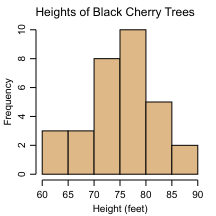
\includegraphics[width=0.5\linewidth]{images/histogram_example.png}
    \caption{Example of a Histogram}
    \label{fig:1}
\end{figure}


\section{Law of large numbers}
As the number of trials (or samples) increases, the sample average (or empirical mean) will converge to the expected value (or population mean).
\subsubsection{Weak Law of large numbers}
The weak law states that the sample average of a sequence of independent identically distributed(i.i.d.) random variables converges in probability to the expected value as the number of samples goes to infinity
$$\bar{X_n} = \frac{1}{n}\sum_{i=1}^{n}X_i \xrightarrow{p} \mu \quad as \ n \to \infty $$
which means, 
$$\forall \varepsilon>0, \lim_{n \to \infty}^n \mathbf{p}(|\bar{X}_n-\mu| > \varepsilon) = 0 $$
\subsubsection{Strong Law of large numbers}
The strong law states that the sample average of a sequence of i.i.d. random variables converges almost surely to the expected value as the number of samples goes to infinity 

$$\bar{X}_n = \frac{1}{n} \sum_{i=1}^n X_i \xrightarrow{a.s.} \mu \quad as\ n \to \infty$$
Which means, 
$$ \mathrm{P}(\lim_{n \to \infty} \bar{X}_n = \mu ) = 1 $$

\section{Central-Limit Theorem}


\section{Measure of Central Tendency} 

\subsection{Mean/Expected Value} 
Average of all data points, sensitive to outliers since a single large outlier could easily skew mean 

$$ \mu = \frac{\sum x_i}{n} $$ 

\subsection{Median}
The middle data point when data are stored, robust to outliers 

\subsection{Mode}
The most frequent data point of the dataset  

\section{Measure of Spread}
Range: Difference between minimum value and maximum value 

$$ Range = x_{max} - x_{min} $$ 

\subsection{Variance}
Average squared deviation, Variance represents Expected variance between mean and data points,
It's basically MSE of a model that just predicts mean, that kinda gives an intutitive 
understanding of how it measures spread

$$\sigma^2 = E[(X - \mu)^2]$$
$$\sigma^2 = E[(X - E[X])^2]$$
$$\sigma^2 = E[X^2]-(E[X])^2$$
$$ \sigma^2 = \frac{\sum (x_i - \mu)^2}{n} (Population) $$ 
$$ s^2 = \frac{\sum( \bar{x_i} - \mu)^2}{n-1} (Sample)  $$ 

\subsection{Standard Deviation}
Root of Variance, 
RMSE of a model that just predicts mean, 
standard deviation gives in intrepretable terms like RMSE

$$ \sigma = \sqrt{\sigma^2} $$
\subsection{Inter Quartile Range(IQR)}
Difference between 75th Percentile/3rd Quartile and 25th Percentile/1st Quartile, 
it is used for outlier detection 
$$IQR = Q_3 - Q_1$$ 
We calculate lower bounds and upper bounds to detect the outliers
$$ \text{lower bound}= Q1-1.5 \times IQR$$
$$ \text{upper bound}= Q3+1.5 \times IQR$$
the data points which values outside of the bounds is considered to be outliers, for more extreme detection \(3 \times IQR\) is also used

\section{Probability Distributions}

\subsection{Discrete Distributions}
A discrete probability distribution describes the probability of occurrence of each value of a discrete random variable
\begin{itemize}
    \item Discrete random variable: Countable values like 1,2,3
    \item Each individual value has an associated probability 
    \item The sum of probabilities for all possible values is 1
    $$ \sum_i \mathrm{P}(X=x_i)=1$$
\end{itemize}

\subsection{Continuous Distributions}

\section{Discrete Probability Distributions}
\subsection{Benoulli Distribution}
The benouli distribution is a discrete probability distribution for a random variable which takes only two possibilities, Sucess or a failure 
\subsubsection{Probability Mass Function(PMF)}
$$
P(X=x) = 
\begin{cases}
    p & \text{if x=1} \\
    1-p & \text{if x=0} \\
    0 & \text{Otherwise}
\end{cases}
$$
Also written as 
$$ \mathrm{P}(X=x) = p^x(1-p)^{1-x}, \quad \text{for x }\epsilon \ \{0,1\}$$

\subsubsection{Statistical Parameters}
\textbf{Mean}\\
Mean is the expected value over many repetitions of the same single-trial experiment,
thus it would be p since, p is probability of 1 appearing and (1-p) is probability of 0 appearing
$$\mu = 1 \times (p)+0 \times (1-p)$$
$$\mu = p$$
\textbf{Variance}\\
Variance can be defined as \( \sigma^2 = E(X^2) - (E(x))^2\), Refer Variance chapter. 
For Bernoulli distribution, \(E(X^2) = p, E(X) = p\), substituting we get
$$\sigma^2 = p - p^2$$
$$\sigma^2 = p(1-p)$$
\textbf{Mode}\\
Mode for Bernoulli would what ever the outcome which is more favored, which can be defined as  
$$
Mode = 
\begin{cases}
    1 & \text{If \(p > 0.5 \)}  \\
    0 & \text{If \(p < 0.5\)}
\end{cases}
$$
\subsubsection{Examples}
\begin{itemize}
    \item Will it rain tomorrow?
    \item Will this patient recover?
    \item Will this product be defective?
\end{itemize}

\begin{figure}[H]
    \centering
    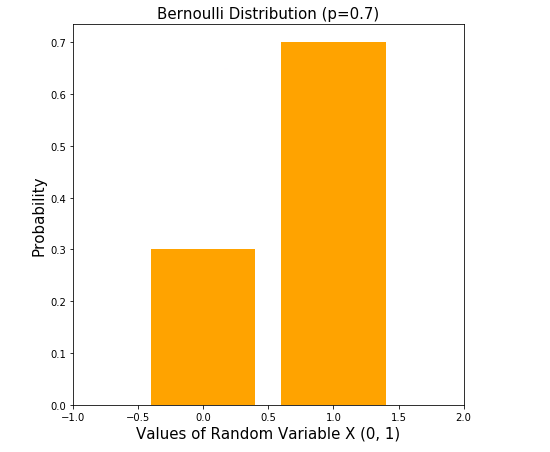
\includegraphics[width=0.5\linewidth]{images/bernoulli_example.png}
    \caption{Example of a Bernoulli Distribution}
    \label{fig:enter-label}
\end{figure}

\subsection{Binomial}
Binomial Distribution is a discrete probability distribution that models the probability of obtaining a specific number of successes
in a fixed number of independent trials(n), these independent trials are just Bernoulli trials, you could see the similarity between
them in statistical parameters

\subsubsection{Probability Mass Function(PMF)}

$$ P(X=x) = nCx \times p^x \times (1-p)^{(n-x)} $$
where,\\
n - no of trials,\\ 
p - probability of success\\
x - number of success\\

\subsubsection{Statistical Parameters}
\textbf{Mean}\\
Mean represents Average number of success from your trails which would be number of trials (n) times probability of success (p)
$$ \mu = n \times p $$
\textbf{Variance}\\
Variance represents Expected variance between mean and data points,
$$ \sigma^2 = n \times p \times (1-p) $$
\textbf{Mode}\\
$$ Mode = 
\begin{cases}
  \text{floor(n+1)p)} & \text{if (n+1)p is not an Integer} \\
  \text{floor((n+1)p), floor((n+1)(1-p))} & \text{if (n+1)p is an Integer} \\
\end{cases}$$ \\
$$ \text{Mode(if p = 0.5)} = 
\begin{cases}
  \frac{n}{2} & \text{if (n+1)p is not an Integer} \\
  \frac{(n-1)}{2},\frac{(n+1)}{2} & \text{if (n+1)p is an Integer} \\
\end{cases}
$$
\subsubsection{Examples}
\begin{itemize}
    \item How many patients will recover out of 50?
    \item How many rainy days this month?
    \item How many defective products in a batch of 1000?
\end{itemize}

\subsection{Negative-Binomial}
\subsection{Multinomial}
\subsection{Geometric}
\subsection{Hypergeometric}
\subsection{Poisson}
\subsection{Discrete Uniform}
\subsection{Normal Distribution}


\subsubsection{Use cases}
\begin{itemize}
    \item When there is only one trial
    \item When the outcome is binary True/False Yes/No 
\end{itemize}




\section{Shape fo the Distributions}
\subsection{Skewness} 
Measure of Asymmetry  
\subsubsection{Right-skewed} 
tail on the right (\(mean > median\)) 

\subsubsection{Left-skewed}
tail on the left (\(mean < median\))

\section{Hypothesis Testing}

\subsection{Null Hypothesis($H_0$)}
Null Hypothesis is the default claim basically means no effect/ no differnce

\subsection{Alternate Hypothesis($H_a$)}
Alternate Hypothesis is the hypothesis that u want to prove

\subsection{One sided Test}
When you have to test if the parameter is greater than or less than the 
hypothesised value, but not both \\
Null:$H_0: \mu = \mu_0 $ \\
Alternate:$H_a: \mu > \mu_0$ or $\mu < \mu_0$

\subsection{Two sided Test}
When you have to test if the parameter is different from the hypothesised value
in either direction
Null:$H_0: \mu = \mu_0 $ \\
Alternate:$H_a: \mu \neq \mu_0$

\subsection{Test Statistic}
A test statistic is a function of the sample data that is used to decide
whether to accept/reject the null hypothesis

$$ \text{Test Statistic} = \frac{\text{How surprised we are}}{\text{How surprised we can be}} $$
$$ \text{Test Statistic} =
\frac{\text{Observed Value - Expected value under $H_0$ }} {\text{Standard Error of observed value}} $$

\subsection{Sampling distribution under $H_0$}
If null hypothesis is true, what would the distribution of my test statistic look like 
across repeated samples. the sample mean/ test statistic follows normal distribution 
thanks to CLT (central limit theorem), we use that to calculate p-value.
\begin{enumerate}
    \item Calculate sample statistic($\bar{x}$,$s^2$)
    \item Compute test statisctic(t-test,z-test...)
    \item Compare the computed test statistic to the corresponding distribution
        to get the p-value
\end{enumerate}

\subsection{p-value}
The p-value is the probability of observing your data assuming the null
hypothesis is true \\
if p is small(p<$\alpha$), we reject null's hypothesis
if p is high(p>$\alpha$), we reject alternate hypothesis

\section{Machine Learning}
Machine learning(ML) is a way of teaching computers to learn patterns
from data and make prediction. 

\subsection{Type of Machine learning}
\begin{itemize}
    \item Supervised Learning
    \item Unsupervised Learning
    \item Reinforcement Learning
    \item Semi-Supervised Learning
\end{itemize}


\section{Types of Data}
\subsection{Qualitative Data}
Describes Qualities, Charesteristics , or categories
\subsubsection{Nominal}
Pure categories without order, 
Example: blood type(A,B,AB,O), brand names
\subsubsection{Ordinal}
Categories with meaningfull order,
Examples: Rank, Survey rating
\subsection{Quantitative Data}
Measureable quantities, Number have meaningfull terms in terms of magnitude
\subsubsection{Discrete}
Countable values, no in-betweens. 
Examples: number of cars
\subsubsection{Continuous}
Countinous measurements; can take any value within a range, 
Examples: Height, weight, temperature

\section{Data Clearning}

\subsection{Define the target variable}
Analyse over all data and pinpoint what you want to predict in the dataset, \\
if your data is discrete like class - classification, \\
if you have a continuous variable - Regression\\
\subsection{Policy Document}
Policy document is a meta data document that defines each column,
A policy document could define type of the data, nullable, pattern of the data,
Range, units, Logical constraints,description... etc
Example:\\
\begin{tabular}{|l|l|l|l|l|l|}
\hline
Column       & Type    & Null & Pattern/Range   & Constraint         & Notes \\ \hline
user\_id     & string  & No   & regex [A-Z0-9]{8} & unique           & id \\ \hline
age\_years   & int     & No   & [0,120]         & --                & cap outliers \\ \hline
gender       & cat     & Yes  & \{M,F,O\}       & --                & harmonize \\ \hline
signup\_date & date    & No   & YYYY-MM-DD      & ≤ churn\_date     & UTC \\ \hline
churn        & binary  & No   & \{0,1\}         & target            & def: 30d leave \\ \hline
income\_inr  & float   & Yes  & [0,1e8] INR     & winsorize top 1\% & currency check \\ \hline
email        & string  & Yes  & regex email     & --                & PII → hash \\ \hline
\end{tabular}

\subsection{Outlier Detection}

\subsubsection{Inter Quartile Range(IQR)}
Difference between 75th Percentile/3rd Quartile and 25th Percentile/1st Quartile, 
it is used for outlier detection 
$$IQR = Q_3 - Q_1$$ 
We calculate lower bounds and upper bounds to detect the outliers
$$ \text{lower bound}= Q1-1.5 \times IQR$$
$$ \text{upper bound}= Q3+1.5 \times IQR$$
the data points which values outside of the bounds is considered to be outliers, for more extreme detection \(3 \times IQR\) is also used

\subsubsection{Z-score}
How far your point is away from the mean in terms of standard deviation
$$ z_i = \frac{x_i - \mu}{\sigma}   $$
if $z_i$ > 3, the point is very unusual and a potential outlier \\
considers all data agove 3 SD as outliers and eliminates it

\subsection{Percentile/Quantile Trimming}
Trim of top and bottom 1-5 percentage fo data, commonly used in competions
to make sure there are no outliers 
\subsection{Domain Rules}
Domain rules like ages should range between 0 - 120, or temperatures
should range between -50 to 60 degrees

\subsection{Impute missing values}
You can either delete the row entierely or chose to impute the missing values
\subsubsection{Numerical data}
\begin{itemize}
    \item small missing values - mean
    \item skewed - median
    \item important values - regression imputation
    \item many missing - add a missign flag (0) or remove the column entirely
    \item if you are not sure you can test all the methods with cross validation 
        and chose a impuation method (recomended for large datasets)
\end{itemize}
\subsubsection{Categorical}
\begin{itemize}
    \item Low cardinatlity(few categories) - Mode impuation
    \item High cardinatlity - Add a new "missing" category
\end{itemize}

\subsubsection{Time series}
\begin{itemize}
    \item Short gaps - forward/backward fill
    \item Long gaps - Interpolation 
    \item seasonal data - seasonal average + Iterpolation(optional)
\end{itemize}
\subsubsection{Images}
take mean or median of the neighbours to fill in the missing pixels, 
or drop the image from the dataset
\subsubsection{Text}
Drop the entire row or add [missing] token

\subsection{Data transformation}
\subsubsection{Standardization}
$$ x_i = \frac{x_i - \mu }{\sigma} $$
\begin{itemize}
    \item used in linear regression, SVM, PCA, K-means
    \item makes mean 0, and std 1
    \item used to standarize all the numerical featuers so 
        that they don't dominate over one another
\end{itemize}

\subsubsection{Min-Max scaling}
$$ x_i = \frac{x_i - min(x)}{max(x)-min(x)} $$
\begin{itemize}
    \item Used in: neural networks, gradient based models, image pixel scaling
    \item Fits everything in [0,1]
    \item Helps model converge faster
\end{itemize}

\subsubsection{Robust scaling}
$$ x_i = \frac{\text{x-median}}{\text{IQR}} $$
\begin{itemize}
    \item Used in Models sensitive to outliers: regression, SVM, KNN
    \item Ignores extreme values, centers around median
    \item Robust to outliers
\end{itemize}

\subsection{Log transformation}
$$ x_i = \text{log}(x+c) $$
\begin{itemize}
    \item used in skewed data(income , population, counts)
    \item used in exponentialisque data to make it more linear
    \item Compresses large numbers, spreads out small ones to make
        distribution closer to normal
\end{itemize}

\subsection{Text processing}
lemmatizaiton and so on

\subsubsection{Lowercasing}
Converts all the letters into lowercase

\subsubsection{Noise Removal}
Remove punctuation, numbers, symbols,stopwords(if not useful)

\subsubsection{Tokenization}
\begin{itemize}
    \item Convert sentence into smaller units token 
    \item example: I like data science = [I,like, data, science]
    \item Tokens are mostly words but not always
\end{itemize}
\subsubsection{Stemming}
\begin{itemize}
    \item chops suffixes from the words
    \item example: "playing" $\to$ "play", "studies" $\to$ "studi"
\end{itemize}

\subsubsection{Lematization}
\begin{itemize}
    \item Advanced form of stemming
    \item reduces to dictionary base form
    \item example: "playing" $\to$ "play", "studies" $\to$ "study"
    \item requires POS(part of speech) tagging, slower but better
\end{itemize}

\subsection{Handling spelling and special entities}
\begin{itemize}
    \item Spelling correction
    \item Handle emojis, mention, hashtags (social media)
\end{itemize}
\subsection{Name Entity Recognition}
\begin{itemize}
    \item NER can be used for censoring sensity information
    \item for extracting NER and use it as features for the algorithms
\end{itemize}

\subsection{Encoding}
\subsubsection{Bag of Words(BOW)}
\begin{itemize}
    \item Bag of words is one-hot encoding for words
    \item Dictionary based bag of words is often used for larger datasets
    \item It represent frequency of words in a vector format
\end{itemize}

\subsubsection{Term frequency-Inverse document frequency (TF-IDF)}
\begin{itemize}
    \item Mesure How important a word is to a document relative to the whole corpus
    \item common words, less importance
    \item Rare document specific word, higher importance
    \item Vectorize a word BOW style and find TF-IDF for each words to form a vector
        which can be used alongside with cosine similarity to find similar documents
    \item Drawbacks - doesn't consider order of the words
\end{itemize}
$$
TFIDF(t, d) = TF(t,d) \times IDF(t)
$$
Term Frequency is defined as number of times term t appears in document d by 
total number terms in the document
$$
TF(t, d) = \frac{f_{t,d}}{\sum_{t' \in d} f_{t',d}}
$$
Inverse Document Frequency is a penalty for words that appear in many documents
$$
IDF(t) = \log \left( \frac{N}{DF(t)} \right)
$$

\subsubsection{Embedding}
\begin{itemize}
    \item Word2vec,embedding models
    \item converts words/sentences to vectors
    \item the embedding enocdes the meaning of the sentence / word
    \item Words similar to each other are near to each other
\end{itemize}


\subsection{Image processing}
\subsubsection{Resizing and Cropping}
Scaling and cropping to have fixed dimension either to ingest the images into 
a fixed pipeline \\
Example: ResNet expects a 224 X 224 

\subsubsection{Normalization/Scaling}
Use Min Max normalization to normzliae 0 - 255 to 0-1, prevents
large gradients, helps faster training

\subsubsection{Grayscale conversion}
Converting RGB(3 channels) to a single channel (greyscalej) reduces data 
complexity/size and noise especially when it doesn't matter to have all the 
channels like xray and so

\subsubsection{Data Augumentation}
Modifying the input data to simulate real world data like flipping/ rotating
the images, cropping, zooming, adjust brightnes, contrast to add noise, 
prevents overfitting and improves generalization

\subsubsection{Noise Recution/Smoothing}
Camera might introduce some random noise in pixels, using a gaussian blur
smoothes the image and let's the model identify patterns instead of noise

\subsubsection{Histogram Equalization}
Histogram Equalization boosts contrast by spreading pixel intensities, it 
redistributes the pixel intensities so that the histogram covers the whole 
range (0-255), used to color correct low light or medical diagnosis photos

\subsubsection{Color Standardization/White balance}
You can either shoot a white/grey photo in the subjects lighting to calculate
white balance or assume average color of your image should be grey and correct 
each channels accordingly

\subsubsection{Segmentation}
Use pretrained segmentation models like Mask R-CNN, U-net, deeplap, to predict
the subjects and create masks for it


\section{Feature engineering and selection}


\section{Supervised Learning}
\section{Unsupervised Learning}



\section{Evaluation Metrics for Regression}

\subsection{Mean Absolute Error}  

$$MAE = \frac{1}{n}\sum{|y_i - \hat{y_i}|}$$ 
\begin{itemize}
    \item Robust to outliers, treats all errors equally doesn’t square the errors like RMSE,MSE..etc 
    \item It’s used when your model can tolerate moderate outliers  
    \item Interpretability - Has same unit as the thing you are predicting/easy to understand 
    \item Gives out constant gradient (bad for gradient based loss function) 
\end{itemize}
 
\subsubsection{Gradient of MAE} 
$$
\frac{d}{d\hat{y}}|y - \hat{y}| = 
\begin{cases} 
+1 & \text{if }  \hat{y} < y \\ 
-1 & \text{if }  \hat{y} > y \\ 
\text{undefined} & \text{if } \hat{y} = y 
\end{cases} 
$$
As you can see no matter how far the error is from true value it always gives a constant gradient as it treats every error as same
stics
\subsection{Mean Squared Error}
$$MSE = \frac{1}{n}\sum{(y_i - \hat{y_i})^2}$$ 
\begin{itemize}
    \item Penalizes large errors/outliers 
    \item Gives out strong gradient signals  
\end{itemize}
\subsubsection{Gradient of MSE}
$$\frac{d MSE}{d\hat{y}} = -\frac{2}{n}(y-\hat{y})$$
It points in the direction of the error, and it grows linearly with size of the error
Larger the gradient, when prediction are more wrong \(\longrightarrow\) model adjusts faster


\subsection{Root Mean Squared Error(RMSE)}  
$$RMSE = \sqrt{MSE}$$ 
\begin{itemize}
    \item It combines interpretability of MAE and sensitive to errors of MSE
    \item It has smooth gradient curves just like MSE, and it's preferred for gradient descent 
\end{itemize}

\subsubsection{Gradient of RMSE}
$$ \frac{d RMSE}{\hat{y_i}} = \frac{1}{n \times RMSE} (\hat{y_i}-y_i)$$
\begin{enumerate}
    \item The gradient strength changes with RMSE, if your RMSE is very large the gradient becomes small, and if your RMSE is very small the gradient becomes large.
    \item It makes RMSE a Non-constantly scaled loss
    \item MSE is preferred over RMSE in training, but RMSE is preferred while reporting for interpretability  
\end{enumerate}

\subsection{R-Square(\(R^2\))}
\(R^2\) is the coefficient of determination. it tells how well your regression model 
explains the variation in the dependent variable(Y) using independent variables(X)
$$R^2 = 1-\frac{SS_{res}}{SS_{tot}}$$
where,
\begin{itemize}
    \item \(SS_{res} = \sum(y_i - \hat{y_i})^2 \to\) Residual sum of squares(error)/MSE
    \item \( SS_{tot} = \sum(y_i - \bar{y_i})^2 \to\) Total sum of squares (total variability)
\end{itemize}
$$R^2 = 1-\frac{ \sum(y_i - \hat{y_i})^2 }{ \sum(y_i - \bar{y_i})^2} $$
Or, it can also be written more intuitively as 
$$ R^2 = 1 - \frac{MSE}{\sigma^2} $$

\begin{itemize}
    \item Let us understand the formula (1-) operator just switches from maximizing to minimizing
so you can ignore that. \\
    \item \(\frac{MSE}{\sigma^2}\) Explains how well our model performs to a model that 
just predicts mean everytime, so if the ratio is 1, then our model is same as the dumb model,
we have to reduce the ratio but the world likes "more the better" approach 
add (1-) operator we have to maximize the error and it's called as \(R^2\) 
\item \(R^2\) ranges from \((-\infty,1]\)
\end{itemize}

\subsection{Adjusted \(R^2\)}
$$ R^2_{adj} = 1 - \left(\frac{(1-R^2)(n-1)}{n-k-1}\right) $$
The above mentioned is textbook formula but we use our simplified 
representation for \(R^2\)
$$ R^2 = 1 - \frac{MSE}{\sigma^2} $$
so, \(R^2_{adj}\) would be
$$ R^2_{adj} = 1 - \frac{MSE_{adj}}{\sigma^2_{adj}} $$
MSE adjusted accounts for the number of freedoms used up to predict the data, 
which is K,represents number of parameters like number of predictors, number of bias
$$ MSE_{adj} = \frac{\sum(y_i-\hat{y_i})^2}{n-k} $$
Variance adjusted for number of freedoms used up which is 1 (mean), 
thus it'd be n-1 insted of n
$$ \sigma^2_{adj} = \frac{\sum(y_i-\mu)^2}{n-1} $$
Substituting we get,
$$ R^2_{adj} = 1 - \left(\frac{MSE}{\sigma^2} \times \frac{n-1}{n-k}\right) $$
where 
\begin{itemize}
    \item n - number of samples/ training samples
    \item k - number of parameters
\end{itemize}

\subsection{Mean Absolute Percentage Error(MAPE)}
MAPE is a metric used to measure accuracy of a predictive model. It expresses the 
prediction error as the percentage of actual values
$$ MAPE = \frac{1}{n}\sum_{i=1}^{n}\left|\frac{y_i-\hat{y_i}}{y_i}\right| \times 100 $$
MAPE is just like MAE but it gives out the error in percentage thus it's easier to intrepret 

\subsection{Huber Loss}
Huber loss is a robust loss function/evaluation metric that has both strengths of MAE and MSE


$$
L_\delta = 
\begin{cases} 
    \frac{1}{2}(y-\hat{y})^2 & \text{for }|y-\hat{y}| \le \delta \\
    \delta \cdot (|y-\hat{y}|-1/2 \delta) & \text{otherwise} \\
\end{cases}
$$
where, 
\begin{itemize}
    \item \( \delta \) is a hyperparameter that controls the behavior between 
        MSE and MAE behavior
\end{itemize}

\subsubsection{Gradient of Huberloss}

\[
\frac{\partial L}{\partial \hat{y}} =
\begin{cases}
-(y - \hat{y}) & \text{if } |y - \hat{y}| \leq \delta \\
-\delta \cdot \operatorname{sign}(y - \hat{y}) & \text{otherwise}
\end{cases}
\]

example graph goes here

\section{Evaluation Metrics for Classification}

\subsection{Basic Terminologies}

\subsubsection{True Positive}
Correctly predicted positive class

\subsubsection{False Positive}
Falsely Predicted Positive class, actually negative

\subsubsection{True Negative}
Correctly predicted negative class

\subsubsection{False Negative}
Falsely predicted negative class, actually positive 

\subsection{Accuracy}
Out of all predictions how many are correct, 
ratio between correct predictions and total predictions is accuracy
$$ Accuracy = \frac{\text{Correct predictions}} {\text{Total predictions}} $$
can also be written as,
$$ Accuracy = \frac{TP+TN}{TP+TN+FP+FN}  $$

\subsection{Precision}
Out of all my positive class prediction how much did I get correctly, 
ratio between correct positive class prediction and total positive class predicted
$$ \text{Precision} = \frac{\text{No of correct positive class predicted}}{\text{No of positive class predicted }} $$
can also be written as,
$$\text{Precision} = \frac{TP}{TP+FP}$$
Use when FP is costly, when you want every positive prediction to be trust worthy, measures reliability

\subsection{Negative Predicted Value (NPV)}
Out of all my negative predictions how much did I get correctly, 
ratio between
$$ \text{NPV} = \frac{\text{No of correct negative class predicted}}{\text{No of negative class predicted }} $$
can also be written as,
$$\text{NPV} = \frac{\text{TN}}{\text{TN} + \text{FN}}$$
Use when FN is costly, when you want every negative class to be trust worthy

\subsection{Recall(TPR)}
Out of all positive cases how many did I predict correctly, also known as True Positive Rate(TPR)
ratio of correctly predicted positive class and total positive cases
$$ \text{Recall} = \frac{\text{No of correctly predicted positive class}}{\text{No of actual positive class}}  $$
$$ \text{Recall} = \frac{TP}{TP+FN}$$
Use when FN is costly/ wrongly classifying , did it recall everything, predict all positive cases

\subsection{Specificity}
Out of all negative cases how many did I predict correctly, Basically Recall for negative class
$$ \text{Specificity} = \frac{\text{No of correctly predicted negative class}}{\text{No of actual negative class}}  $$
$$ \text{Specificity} = \frac{TN}{TN+FP}$$
Use when FP is costly, when predicting negative class is important

\subsection{False Positive Rate(FPR)}
Out of all negative cases how many did I fail to predict, 
$$ \text{FPR} = \frac{No of wrongly predicted negative class}{No of actual Negative class} $$
$$ \text{FPR} = \frac{FP}{TN+FP} $$
$$ \text{FPR} = 1 - \text{specificity}$$

\subsection{F-score}
It's a harmonic mean between precision and recall

$$F_\beta = \frac{(1 + \beta^2) \cdot \text{Precision} \cdot \text{Recall}}{(\beta^2 \cdot \text{Precision}) + \text{Recall}}$$
\subsubsection{Derivation} 
$$ \frac{1}{F_\beta} = \frac{w_p}{\text{Precision}} + \frac{w_r}{Recall} $$
We want harmonic ratio of precision and recall, 
$$ \frac{w_r}{w_p} = \beta^2$$
We want the weights to add up to one
$$ w_r + w_p = 1 $$
By solving we get
$$ w_r = \frac{\beta^2}{1 + \beta^2} $$ 
$$ w_p = \frac{1}{1 + \beta^2} $$

\section{AUC-ROC curve}
\subsection{Receiver Operating Characteristic (ROC)}
The ROC curve plots the True Positive Rate(TPR) vs False Positive Rate(FPR) at various threshold settings,
it let's you decide which one is best for you based on your requirement
\subsection{Area Under the Curve (AUC)}
The AUC tells how much of the curve is under the line,
usually compared with other models\\
Higher AUC = Better model performance \\

\begin{table}[H]
    \centering
    \begin{tabular}{|c|c|}
        \hline
        Auc Score & Intrepretation \\
        \hline
         0.5 &  Random guessing \\
         0.7 - 0.8 & Acceptable \\
         0.8 - 0.9 & Excellent \\
         \textgreater 0.9 & Outstanding\\
         \hline     
    \end{tabular}
\end{table}

\section{Regularization}
Regularization adds a penalty for complexity to prevent overfitting, make model simpler
$$\text{Regularized Loss} = \text{Loss + Regularization parameter}$$

\subsection{L1}
L1 adds the sum of absolute value of coefficients to the loss function, 
it is used for feature selection since it encourages the optimizer to shirnk
unwanted features to zero
$$\text{L1} = \lambda \sum|w_i| $$

\subsection{L2}
L2 adds teh sum of coefficient squares to the loss function this 
makes the gradient strength smooth, thus it won't reduce everything 
to zero, but towards zero, use it when you think all features contribute
to ur model

$$ \text{L2} = \lambda \sum w_i^2 $$

\subsection{Elastic net}
It's a combination of L1 and L2 where you want to have both sparsity(l2) 
and stability(l2)
$$ \text{Elastic Net} = \alpha \text{L1} + (1-\alpha)\text{L2} $$


\section{Time Series}


\section{TODOO}
\begin{enumerate}
    \item pca
    \item complete the Distributions, some intro to probability
    \item Time series, ML, other stuff

\end{enumerate}

\end{document}
